%%FRAGEN:
%FIT UND PARAMETER EXTREM NAH AN GLEICHRICHTER??
\subsection{Schaltung mit Noise Generator}
\label{sec:mit_noise}
Wie in Schaltplan \textbf{PLAN REFERENZIEREN!!!} dargestellt wird über den Noise Generator ein Rauschsignal hinzu gegeben.
Das Signal ist von der gleichen Größenordnung wie die Signalspannung $U_\text{sig}$.
Der Gain Regulierer am Verstärker ist nun auf 5 gestellt, die Noise Amplitude und der Noise Attenuator auf $10^{-3}$.
Der Gain Regulator des Lock-in Detektors steht weiterhin auf 20.
Analog zu Abschnitt \ref{sec:ohne_noise} werden alle Messungen wiederholt, erst ohne und dann mit Integrationsglied.


\subsubsection{Ohne Tiefpass}
\label{sec:mit_noise_ohne_tp}
Für die Messreihe ohne Integration durch den Tiefpass ergeben sich die Spannungsverläufe \ref{fig:phasenunterschiede_mit_noise}.
Im Vergleich zu den Signalen in Abbildung \ref{fig:phasenunterschiede_ohne_noise} ist erkennbar, dass bei gleicher Siganlspannung $U_\text{sig}$
die Signale am Oszilloskop die gleiche Form (augenscheinlich gleiche Frequenz und Amplitude) haben.
Die einzige Ausnahme ist hierbei das Bild von $\phi = \qty[]{180}{\degree}$ (vgl. \ref{fig:phase5} und \ref{fig:phase10}).
Verglichen mit den Abbildungen im Anhang sieht es allerdings so aus, als wäre versehentlich bei der Durchführung mit dem Noise Generator eine Phase von 
\qty[]{270}{\degree} eingestellt worden, wodurch sich diese Diskrepanz erklären lässt.
%
%
\begin{figure}[H]%
    \begin{subfigure}{0.5\textwidth}%
    \centering%
    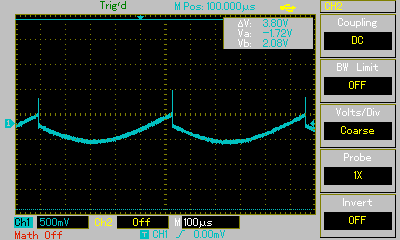
\includegraphics[width = 7.3cm]{./Oszilloskop Bilder/png/5.3/n1.png}%
    \caption{$\phi = \qty[]{0}{\degree}$}%
    \label{fig:phase6}%
    \end{subfigure}%
    %
    \hfill% Fills available space in the center -> space between figures
    \begin{subfigure}{0.5\textwidth}%
    \centering%
    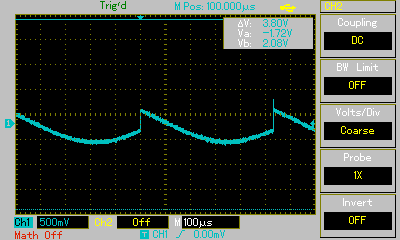
\includegraphics[width = 7.3cm]{./Oszilloskop Bilder/png/5.3/n2.png}%
    \caption{$\phi = \qty[]{45}{\degree}$}%
    \label{fig:phase7}%
    \end{subfigure}%
    %
    \hfill
    \begin{subfigure}{0.5\textwidth}%
    \centering%
    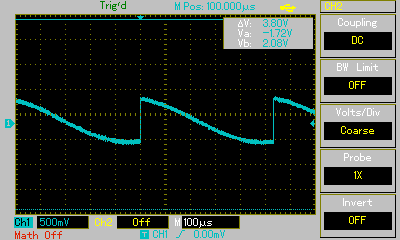
\includegraphics[width = 7.3cm]{./Oszilloskop Bilder/png/5.3/n3.png}%
    \caption{$\phi = \qty[]{90}{\degree}$}%
    \label{fig:phase8}%
    \end{subfigure}%
    %
    \hfill% Fills available space in the center -> space between figures
    \begin{subfigure}{0.5\textwidth}%
    \centering%
    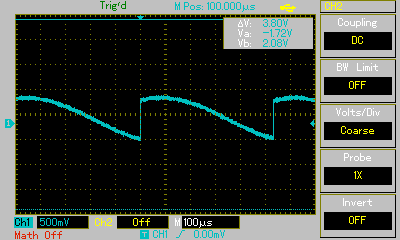
\includegraphics[width = 7.3cm]{./Oszilloskop Bilder/png/5.3/n4.png}%
    \caption{$\phi = \qty[]{135}{\degree}$}%
    \label{fig:phase9}%
    \end{subfigure}%
    %
    \hfill
    \begin{subfigure}{0.5\textwidth}%
    \centering%
    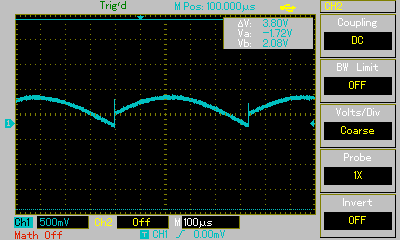
\includegraphics[width = 7.3cm]{./Oszilloskop Bilder/png/5.3/n5.png}%
    \caption{$\phi = \qty[]{180}{\degree}$ (laut Notizen)}%
    \label{fig:phase10}%
    \end{subfigure}%
    %
    \caption{Spannungsverläufe für unterschiedliche Phasen ohne Integration mit Noise Generator}%
    \label{fig:phasenunterschiede_mit_noise}%
\end{figure}%


\subsubsection{Spannung in Abhängigkeit der Phase nach Integration mit Geräuschen}
Unter Verwendung des Tiefpasses ergeben sich abhängig von der Phasenverschiebungen $\phi$ die Spannungen
$U_\text{noise}$ in \ref{tab:u_noise}.
%
\begin{table}
    \centering
    \caption[]{Ausgangsspannung nach Integration mit Geräuschsignal}
    \label{tab:u_noise}
    \sisetup{table-format=3.0}
    \begin{tabular}[]{S c S[table-format=2.2]}
        \toprule
        {$\phi / \unit[]{\degree}$} & {$\phi / \unit[]{\radian}$} & {$U_\text{noise} / \unit[]{\volt}$} \\
        \midrule
           0 &     0          & -0.18 \\ % Ch1 Ampl in V: 1.11
          45 & $    \pi / 4 $ & -0.16 \\ % Ch1 Ampl in V: 0.7722
          90 & $    \pi / 2 $ &  0.00 \\ % Ch1 Ampl in V: 0.9306
         135 & $ 3  \pi / 4 $ &  0.22 \\ % Ch1 Ampl in V: 0.8910
         180 & $    \pi     $ &  0.34 \\ % Ch1 Ampl in V: 0.6138
         225 & $ 5  \pi / 4 $ &  0.32 \\ % Ch1 Ampl in V: 0.9306
         270 & $ 3  \pi / 2 $ &  0.16 \\ % Ch1 Ampl in V: 1.33
         300 & $ 5  \pi / 3 $ &  0.04 \\ % Ch1 Ampl in V: 1.49
         315 & $ 7  \pi / 4 $ & -0.04 \\ % Ch1 Ampl in V: 1.45
         330 & $ 11 \pi / 6 $ & -0.12 \\ % Ch1 Ampl in V: 1.21
        \bottomrule
    \end{tabular}
\end{table} 
Analog zu Abschnitt \ref{sec:integration_ohne_noise} ergeben sich mit der Ausgleichsfunktion \eqref{eq:ausgleich_tp_ohne_noise} die Parameter
\begin{align*}
    A_\text{noise} &= \left(\num[]{-0.2747} \pm \num[]{0.0055}\right) \, \unit{\volt} & B_\text{noise} &=  \num[]{0.9933} \pm \num[]{0.0150} \\
    C_\text{noise} &= \num[]{-0.2754} \pm \num[]{0.0564} & D_\text{noise} &= \left(\num[]{0.0810} \pm \num[]{0.0054}\right) \, \unit[]{\volt}.
\end{align*}
Auch hier errechnen sich die Fehler auf die Parameter durch die Kovarianzmatrix.
%param_a = ufloat(-0.27466768, 0.00545352)
%param_b = ufloat(0.99333910 , 0.01503098)
%param_c = ufloat(-0.27544268, 0.05641517)
%param_d = ufloat(0.08103079 , 0.00536591)
\begin{figure}[H]
    \includegraphics[]{build/B02_ausgleichsplot.pdf}
    \caption[]{Ausgleichsfunktion \eqref{eq:ausgleich_tp_ohne_noise} zu den Werten aus Tabelle \ref{tab:u_noise}}
    \label{fig:ausgleichsplot2}
\end{figure}

\noindent
Es ist leicht erkennbar, dass die beiden Ausgleichsfunktionen nah bei einander liegen. 
Da allerdings der Gain Regulator am Verstärker um den Faktor 5 größer als zuvor eingestellt ist,
folgt für die Amplitude der Eingangsspannung ein Wert von 
\begin{align*}
    U_{0,\text{noise}} = \frac{\pi}{2} \frac{1}{5 \cdot 20} A_\text{noise} = \left(-4.31 \pm 0.09\right) \, \unit[]{\milli\volt},
\end{align*}
was einem Verhältnis von $\Delta U_{0,\text{noise}} = \left(43.1 \pm 0.9\right) \, \%$ im Vergleich zu $U_0$ entspricht.
Im Vergleich zu vorher gibt es somit einen Unterschied von $\frac{U_{0,\text{out}}}{U_{0,\text{noise}}} = \left(3.64 \pm 0.12\right)$.
%\begin{align*}
%    \frac{U_{0,\text{out}}}{U_{0,\text{noise}}} = \left(3.64 \pm 0.12\right).
%\end{align*}

%#U_0_noise =  -0.00431+/-0.00009
%#delta u_noise =  0.431+/-0.009
%abweichung out noise :  3.64+/-0.12

